\chapter{Studi Literatur}

  Pada bab ini akan dipaparkan mengenai beberapa penelitian terkait deteksi intrusi paralel berbasis GPU yang telah dilakukan sebelumnya berikut metodologi serta ketercapaian yang didapatkan. Selain itu, pada bab ini juga akan dijelaskan lebih lanjut mengenai landasan teori dari pengerjaan tugas ini.


\section{Deteksi dan Pencegahan Intrusi}

  \subsection{Deteksi Intrusi}

    Intrusi merupakan serangkaian percobaan yang tidak berhak, baik sukses maupun tidak, untuk menyusup masuk, mengakses, mengubah, atau menyalahgunakan sumber daya yang berharga sehingga sumber daya menjadi tidak dapat dipercaya atau bahkan digunakan \parencite{kizza2015}. Proses intrusi sistem terbagi menjadi beberapa tahap. Proses dimulai dengan identifikasi target. Lalu target akan diperiksa secara menyeluruh dan dicari celah keamanannya. Selanjutnya dilakukan pengambilalihan akses ke sistem. Dan terakhir, sumber daya dalam sistem dapat dibaca, digunakan dan dimodifikasi. 

    Deteksi intrusi adalah kegiatan merekam, menganalisa, dan mendeteksi kemungkinan sebuah percobaan akses yang tidak berhak terhadap sebuah sistem \parencite{kizza2015}. Adanya percobaan akses ilegal dapat mengindikasikan adanya serangan dari luar (\emph{hijacking}), maupun dari dalam (seperti \emph{malware}). Setelah serangan ditemukan, aktivitas akan dicatat ke log untuk ditindak lebih lanjut.

    Selain deteksi intrusi, kegiatan yang berkaitan adalah pencegahan intrusi. Pencegahan intrusi merupakan deteksi intrusi yang secara aktif melakukan penyaringan terhadap percobaan akses ke sistem. Jika terindikasi sistem terkena percobaan serangan, maka semua percobaan akses yang terkait akan dihentikan. Tindakan lebih lanjut yaitu aliran paket bisa diblok baik untuk sementara waktu maupun secara permanen.

  \subsection{Sistem Deteksi dan Pencegahan Intrusi}

    Sistem deteksi dan pencegahan intrusi (\emph{intrusion detection and prevention system} abbr IDPS) adalah mekanisme yang mengotomasi proses deteksi dan pencegahan intrusi kepada satu atau beberapa node. Sistem mengambil paket yang masuk sambil melakukan pengecekan kemudian membuat laporan hasil inspeksi. Laporan hasil inspeksi dapat digunakan untuk menentukan aksi yang akan dilakukan pada paket \parencite{nist2007}.

    Ada dua macam NIDPS dilihat dari cakupan deteksinya:
    \begin{enumerate}

      \item 
      \emph{Network Based IDPS (NIDPS)} \\
      IDPS tipe ini dapat melakukan analisis aliran paket dalam suatu subnet jaringan. IDPS ini biasanya diletakkan di sebuah segment jaringan seperti \emph{gateway}, \emph{hub / switch}, \emph{router}, dsb. Cara kerja NIDPS mirip dengan \emph{network sniffer}, yaitu mengambil seluruh paket yang berjalan pada jaringan. IDPS jenis ini digunakan untuk mengantisipasi serangan jenis DoS (\emph{denial of service}) dan \emph{network probing}.

       \item 
      \emph{Host Based IDPS (HIDPS)} \\
      IDPS tipe ini dapat mengambil seluruh informasi pada sistem operasi seperti \emph{audit trails}, \emph{logs}, \emph{system logs}, dsb dan melakukan analisis terhadap perilaku sistem. IDPS jenis ini digunakan untuk mengantisipasi serangan yang menargetkan sistem operasi, seperti \emph{buffer overflow}, \emph{malware}, dll.

    \end{enumerate}

    Fokus tugas akhir ini akan membahas tentang NIDPS.

  \subsection{Metode Deteksi Intrusi}

    Ada tiga macam metode deteksi yang biasa dipakai dalam NIDPS:
    \begin{enumerate}

      \item
      \emph{Signature-based Detection} \\
      \emph{Signature} adalah pola aktivitas tertentu yang mengindikasikan adanya ancaman. IDS berbasis \emph{signature} melakukan pencocokan \emph{signature} dengan aktivitas sistem untuk mengidentifikasi insiden yang mungkin. Pengenalan berbasis \emph{signature} sangat efektif dan cepat untuk mendeteksi ancaman yang telah dikenal. Tapi metode ini tidak efektif untuk mendeteksi ancaman yang belum pernah dikenal sebelumnya atau ancaman yang disamarkan dengan teknik-teknik tertentu.

      Metode ini adalah metode termudah karena hanya membandingkan unit aktivitas saat ini, seperti paket atau \emph{log entry}, dengan daftar \emph{signature} menggunakan operasi perbandingan string. Selain itu jumlah \emph{false alarm} yang dihasilkan juga relatif sedikit. Metode berbasis \emph{signature} membutuhkan sedikit pengetahuan tentang protokol jaringan dan aplikasi, dan tidak dapat melacak atau mendapat state dari komunikasi yang kompleks.

      \item
      \emph{Anomaly-based Detection} \\
      IDS berbasis anomali melakukan analisis parameter aktivitas yang dianggap normal dengan aktivitas sistem sekarang untuk melihat penyimpangan yang signifikan. Sistem menggunakan profil untuk menentukan parameter aktivitas normal seperti user, host, koneksi jaringan, atau aplikasi. Profil dikembangkan menggunakan pembelajaran mesin dengan memantau karakteristik dari aktivitas sejenis selama selang waktu tertentu.

      Sistem akan menggunakan metode statistik untuk membandingkan karakteristik aktivitas sekarang terhadap batas yang terkait dengan profil. Ketika ada aktivitas yang menyimpang cukup jauh dari batas, akan dicatat ke log dan dilaporkan ke \emph{administrator} / pengelola. Profil bisa dikembangkan dari berbagai atribut, seperti jumlah email yang dikirim oleh pengguna, jumlah percobaan login yang gagal, dan tingkat penggunaan CPU host waktu tertentu.

      Keuntungan dari metode berbasis anomali ini adalah dapat mendeteksi ancaman yang belum pernah dikenal sebelumnya. Contoh, sebuah proses yang menggunakan sumber daya dalam jumlah besar, mengirim banyak email, menjalankan banyak koneksi, dan melakukan kegiatan lain yang cukup berbeda dari profil sistem normal akan terdeteksi sebagai \emph{malware}.

      Profil awal dibangkitkan selama rentang waktu tertentu yang disebut \emph{training period}. Kemudian profil dapat diperbarui secara statis atau dinamis. Dinamis ketika profil diperbarui dengan log aktivitas sistem. Statis jika profil diperbarui secara manual.

      \item
      \emph{Stateful Protocol Analysis} \\
      \emph{Stateful protocol analysis} atau analisis protokol dengan \emph{state} adalah proses membandingkan profil yang telah ditentukan sebelumnya terhadap definisi aktivitas protokol yang dianggap tidak berbahaya dan berlaku umum untuk setiap protokol. Profil diukur terhadap batas tertentu untuk mengidentifikasi penyimpangan. 

      Tidak seperti deteksi berbasis anomali, yang menggunakan profil khusus host atau jaringan, analisis protokol dengan \emph{state} bergantung pada profil universal yang dikembangkan vendor yang menentukan bagaimana protokol tertentu seharusnya dan tidak boleh digunakan. Contoh, saat pengguna memulai sesi \emph{File Transfer Protocol} (FTP), sesi awalnya dalam \emph{state} yang tidak terotorisasi. Pengguna yang tidak terotorisasi hanya dapat melakukan beberapa perintah di \emph{state} ini, seperti melihat informasi umum dan memberikan nama pengguna dan kata sandi. 

      Bagian penting dari pengenalan \emph{state} adalah mencocokkan \emph{request} dengan respons, jadi ketika upaya otentikasi FTP terjadi, IDS dapat menentukan apakah berhasil dengan menemukan kode \emph{state} dalam respons yang sesuai. Setelah pengguna berhasil dikonfirmasi, sesi diset berada dalam keadaan terotentikasi, dan pengguna dapat melakukan lebih banyak perintah. Contohnya adalah jika terlalu banyak perintah dalam suatu \emph{request} dilakukan dalam \emph{state} yang tidak diotentikasi, maka akan dianggap mencurigakan. 

    \end{enumerate}

    Selain ketiga kategori di atas, penggunaan metode deteksi \emph{hybrid} \emph{signature-based} dan \emph{anomaly-based} menjadi populer karena fleksibilitas dan kinerjanya. Cakupan dari \emph{signature-based} NIDPS dapat ditingkatkan dengan \emph{rule} baru hasil pembelajaran dari model \emph{anomaly-based}.

\section{Snort NIDPS}

    Snort NIDPS adalah sistem deteksi dan pencegahan intrusi yang mampu melakukan analisis lalu lintas secara \emph{real-time} dan \emph{logging} paket dalam jaringan \parencite{snortfaq}. Snort mampu melakukan eksekusi \emph{rule} untuk deteksi lalu lintas yang berbahaya dan melaporkan ke pengelola. \emph{Rule} dibentuk berdasarkan perbedaan protokol paket dalam jaringan. \emph{Rule} ini kemudian digunakan untuk melakukan analisis protokol dan pencocokan \parencite{snort}. Kumpulan \emph{rule} ini kemudian disebut juga kebijakan (\emph{policies}). 

  \subsection{Modus Snort NIDPS}

    Snort memiliki 3 buah modus, modus pengendus, modus pencatat, dan modus deteksi intrusi. Modus pengendus hanya menampilkan informasi tentang \emph{header} paket. Perintah yang berbeda dapat digunakan menampilkan \emph{header} untuk protokol berbeda. Modus pencatat hanya mencatat paket ke disk. Modus ini dapat digunakan untuk menggolongkan payload berdasarkan protokol dalam direktori yang berbeda. Dan terakhir, modus deteksi intrusi akan melakukan deteksi intrusi dari paket yang disimpan maupun analisis lalu lintas jaringan secara realtime. Modus ini dikonfigurasi menggunakan sebuah file konfigurasi \parencite{snortfaq}. Melalui modus ini, Snort juga dapat dikonfigurasi agar menjadi sistem pencegah intrusi (NIPS) untuk menghalangi jaringan dengan membuat sebuah \emph{bridge} \parencite{snort}.

  \subsection{Implementasi Snort NIDPS}

    Snort memliki beberapa modul; modul penangkap paket, modul \emph{decoder}, modul preproses, modul detektor, dan modul keluaran. Modul penangkap bertujuan mengambil paket dari lalu lintas jaringan. Lalu paket akan diproses dengan modul \emph{decoder} akan mengidentifikasi protokol paket dan mengklasifikasikannya berdasarkan spesifikasi data-link. Preproses bertujuan mengolah paket berdasarkan jenis protokol paket untuk kemudian siap dideteksi. Preproses juga bertujuan menyusun fragmen IP dan \emph{stream} TCP. Selain itu paket juga dicek jika berada diluar TCP \emph{window}, dan akan dikembalikan sehingga bisa disusun ulang \parencite{snort}. Lalu terakhir, paket akan dicek oleh modul detektor menggunakan \emph{rule} yang tersedia dan mengirimkan hasilnya ke modul keluaran. Saat ini Snort hanya mengimplementasi modul detektor pada \emph{single thread} CPU. Sehingga performa maksimum Snort hanya sekitar 200-300 Mbps \parencite{albin2012}.

  \subsection{\emph{Rule} Snort NIDPS}

    \emph{Rule} adalah kumpulan kata kunci yang digunakan dalam deteksi kemungkinan pelanggaran kebijakan keamanan. Snort akan melakukan pencocokan paket berdasarkan kondisi yang dispesifikasikan dalam tiap \emph{rule}. \emph{Rule} memiliki struktur dasar berupa \emph{header} dan \emph{body} \parencite{snort}. 

    \emph{Header} berisi spesifikasi dari  \emph{rule} berupa aksi, protokol, IP sumber, port sumber, operator, IP tujuan, port tujuan. Operator menandai arah dari paket. Arah paket bisa satu atau dua arah. Aksi akan dijalankan jika signature paket cocok dengan \emph{rule} \parencite{5358130}. Sedangkan \emph{body} \emph{rule} berisi kumpulan \emph{option} yang digunakan untuk pencocokan paket. 

    \begin{figure}[H]
      \centering
      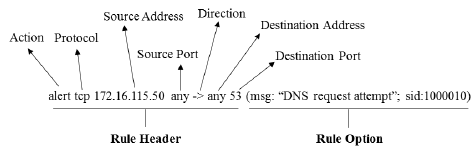
\includegraphics[width=0.8\textwidth]{resources/rule.png}
      \caption[Struktur \emph{rule} Snort NIDPS]{Struktur \emph{rule} Snort NIDPS \parencite{khamphakdee2014}}
    \end{figure}

    Beberapa \emph{option} yang biasa digunakan dalam Snort \emph{Rule} diantaranya:
    \begin{enumerate} 
      \item \emph{sid}, ID \emph{rule}
      \item \emph{msg}, pesan kesalahan yang ditampilkan ke pengelola atau log
      \item \emph{flow}, arah aliran paket dari atau ke server
      \item \emph{flags}, flag TCP yang dicari
      \item \emph{content}, konten yang dicocokkan berupa teks
      \item \emph{reference}, acuan \emph{vulnerability} yang diduga
    \end{enumerate} 

\section{\emph{Pattern Matching}}

  \emph{Pattern matching} adalah metode mencari kemunculan sebuah string atau substring terhadap string lain. \emph{Pattern matching} menjadi operasi paling kritis dan sangat berpengaruh dalam kinerja NIDPS. Ada dua jenis utama pencocokan pola, yaitu \emph{single pattern matching} dan \emph{multi-pattern matching}. Fokus bahasan tugas akhir ini adalah \emph{multi-pattern matching}.

  \subsection{Algoritma Aho-Corasick}

    Algoritma Aho-Corasick adalah algoritma \emph{multi-pattern matching} yang dapat mencari kemunculan string dalam sebuah kamus \parencite{ahoc1975}. Pencarian juga bisa dilakukan pada substring terhadap semua string dalam kamus. Dengan memodelkan pola paket menjadi string atau regular expression, dapat dicari kemunculan pola serangan menggunakan algoritma Aho-Corasick ini.

    Kamus berisi semua string \emph{rule} yang akan dicocokkan. Pembangkitan kamus hanya dilakukan sekali sebelum pencocokan string dilakukan. Ada beberapa desain kamus yang dapat digunakan. Salah satu bentuk yang umum yaitu \emph{finite automata} atau FSM (\emph{finite state machine}) yang menyerupai \emph{trie}. Pembangkitan kamus dapat dilakukan dalam $O(kp)$, dengan $k$ adalah jumlah string pada kamus dan $p$ adalah panjang maksimum string pada kamus.

    \begin{figure}[H]
      \centering
      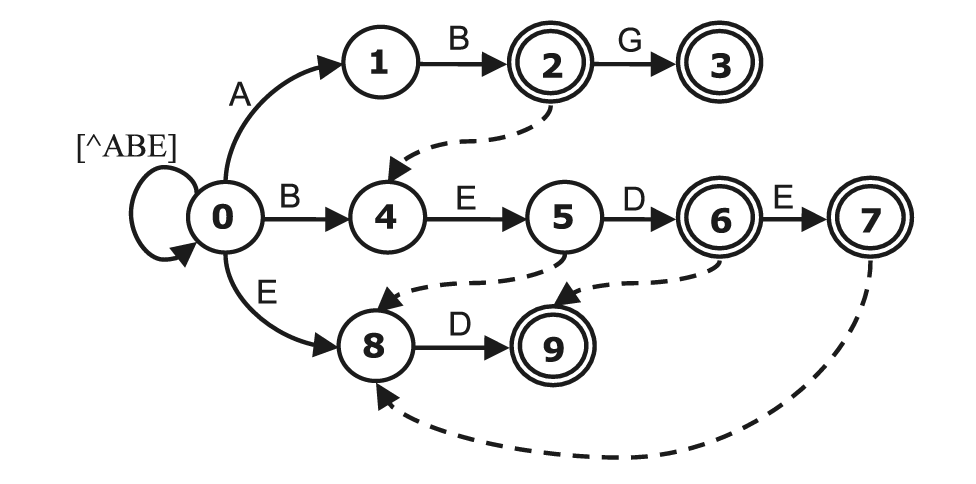
\includegraphics[width=0.6\textwidth]{resources/aho-c.png}
      \caption[\emph{Finite automata} kamus algoritma Aho-Corasick dengan \emph{failure transition}]{\emph{Finite automata} kamus algoritma Aho-Corasick dengan \emph{failure transition} \parencite{lin2013}}
    \end{figure}

    \emph{Trie} adalah pohon yang menggambarkan urutan karakter prefiks dalam beberapa string \parencite{trie59}. \emph{Trie} akan dimulai dari simpul kosong. Lalu bercabang hanya jika ada huruf yang berbeda. Sehingga pencarian string dalam kamus hanya dilakukan dengan menelusuri tiap simpul pada \emph{trie}. 

    Desain yang lebih padat menggunakan \emph{failure transition}. \emph{Failure transition} akan menunjuk ke posisi terakhir prefiks yang cocok dengan suffiks string yang dicari. Sehingga ketika pencarian tidak cocok pada suatu string, akan dilanjutkan pada string berikutnya yang prefiksnya cocok dengan suffiks string sebelumnya. Menggunakan \emph{failure transition}, pencocokan banyak pola dapat lebih efisien ketimbang harus mengulang tiap pencarian dari awal. Sehingga pencarian dapat dilakukan dalam $O(x)$, dengan $x$ adalah panjang string pola.

  \subsection {\emph{Parallel Failureless Aho-Corasick}}

    Untuk dapat meningkatkan kinerja algoritma Aho-Corasick, kamus dapat dipartisi menjadi beberapa segmen untuk tiap pola. Sehingga tiap partisi dapat digunakan untuk pencocokan pada tiap \emph{thread}. Namun terdapat ada masalah pada pencocokan partisi ketika pola yang dicari ternyata berada pada lebih dari satu partisi dan terpotong. Hal ini dikenal sebagai \emph{boundary detection problem}. Sehingga, pencarian perlu untuk mengiterasi string sebelumnya dan meningkatkan \emph{runtime secara} drastis.

    Maka, dikembangkan sebuah modifikasi algoritma Aho-Corasick yang mampu melakukan partisi dan pencocokan tanpa mengalami masalah seperti di atas yang disebut \emph{Parallel Failureless Aho-Corasick} (PFAC). PFAC menggunakan \emph{state machine} yang tidak mengandung \emph{failure transition} dan masing-masing \emph{thread} hanya mencocokkan satu string pola \parencite{lin2013}. Menggunakan desain ini, PFAC lebih hemat memori karena tidak menggunakan \emph{failure transition}. Selain itu, umur \emph{thread} juga lebih singkat sehingga \emph{throughput} yang dihasilkan lebih besar.

    \begin{figure}[H]
      \centering
      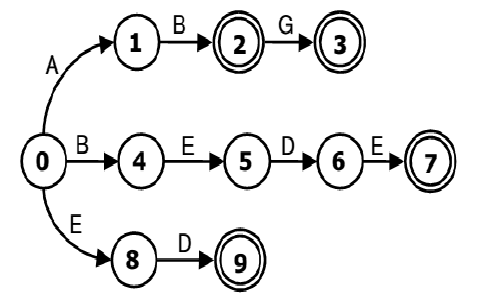
\includegraphics[width=0.5\textwidth]{resources/pfac.png}
      \caption[\emph{Finite automata} Aho-Corasick tanpa \emph{failure transition}]{\emph{Finite automata} Aho-Corasick tanpa \emph{failure transition} \parencite{lin2013}}
    \end{figure}

\section{\emph{General-Purpose computing on Graphics Processing Units}}

  \emph{General-purpose computing on graphics processing units} (GPGPU, kadang disebut juga GPGP atau GP\textsuperscript{2}U) adalah teknik untuk menggunakan pemroses grafis / GPU untuk melakukan komputasi umum yang biasa dilakukan pada pemroses CPU. GPU memiliki banyak core yang berjalan paralel. Desain GPU berbeda dari CPU karena fokus GPU adalah melakukan operasi secara paralel. Berbeda dari CPU yang digunakan untuk melakukan operasi sekuensial \parencite{lindholm2001}. Dalam GPU terdapat beberapa \emph{stream processor} yang masing-masing memiliki beberapa \emph{core thread}.

  \begin{figure}[H]
    \centering
    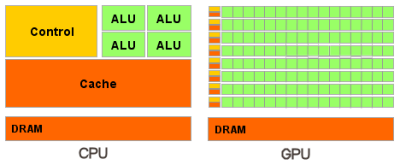
\includegraphics[width=0.8\textwidth]{resources/GPUvsCPU.png}
    \caption[Perbedaan arsitektur CPU dan GPU]{Perbedaan arsitektur CPU dan GPU \parencite{cuda}}
  \end{figure}

  Penelitian tentang GPGPU dimulai ketika \emph{programmable pixel} dan \emph{vertex shaders} diperkenalkan. Penggunaan GPGPU lebih mudah dengan adanya \emph{shading language} yang berjalan pada GPU. \emph{Shading language} adalah bahasa pemrograman yang spesifik untuk mendeskripsikan tampilan sebuah \emph{scene} \parencite{proudfoot2001}. \emph{Shading language} bertujuan menyediakan antarmuka \emph{high level} untuk operasi \emph{vertex} pada GPU. 

  Dengan adanya \emph{shading language}, operasi vektor dan matriks dapat dengan mudah diubah menjadi operasi \emph{vertex}. Sejak saat itu, usaha untuk melakukan komputasi umum dengan GPU mulai bermunculan seperti perkalian matriks \parencite{matrix2001}, simulasi fisika \parencite{phys2002}, hingga dekomposisi LU pada matriks persegi \parencite{lugpu2005}. Maka, pada tahun 2003, dalam disertasinya \parencite{harris2003}, Mark Harris mengajukan sebuah istilah yang kini dikenal sebagai \emph{general-purpose computing on graphics processing units} (GPGPU) sekaligus mendirikan situs GPGPU.org.

  Saat ini ada dua platform GPGPU yang populer, CUDA dan OpenCL. CUDA adalah platform yang dikembangkan oleh NVIDIA. CUDA hanya dapat berjalan pada GPU NVIDIA. Sedangkan OpenCL dikembangkan oleh konsorsium Khronos Group. OpenCL dapat berjalan pada banyak perangkat, seperti CPU, GPU, FPGA, dan DSP (\emph{digital signal processor})).

  \subsection{\emph{Compute Unified Device Architecture}}

    \emph{Compute Unified Device Architecture} (CUDA) adalah platform dan API untuk GPGPU oleh NVIDIA. CUDA menyediakan antarmuka untuk dapat menggunakan GPU NVIDIA untuk melakukan GPGPU \parencite{cuda}. CUDA API dapat diimplementasi menggunakan bahasa C, C++, dan Fortran. Selain itu, ada juga binding yang dibuat dalam pustaka beberapa bahasa oleh pihak ketiga, seperti Python, Perl, Java, Ruby, Haskell, Lua, MATLAB, dan Mathematica.

    \subsubsection{Struktur Kode CUDA}

      Terdapat dua perangkat yang berbeda untuk \emph{runtime} CUDA, yaitu \emph{host} (CPU), dan \emph{device} (GPU). Masing-masing platform akan menjalankan bagian kode tersendiri. Ada dua bagian dalam kode program CUDA, yaitu \emph{host code} dan \emph{kernel code}. Ketika program berjalan, maka \emph{host code} akan berjalan terlebih dahulu. Lalu, \emph{kernel code} akan disalin dan dijalankan di memori GPU. Karena memori yang dapat diakses oleh masing-masing kode juga terpisah, maka perlu dilakukan alokasi pada memori \emph{device} dan transfer antar memori \emph{device} dan memori \emph{host}.

    \subsubsection{\emph{CUDA Thread}}

      CUDA \emph{thread} dibagi menjadi beberapa kelompok blok yang disebut \emph{grid}. Masing-masing \emph{grid} berisi beberapa buah blok. Di dalam blok terdapat beberapa \emph{thread} yang akan berjalan terpisah. 

      \begin{figure}[H]
        \centering
        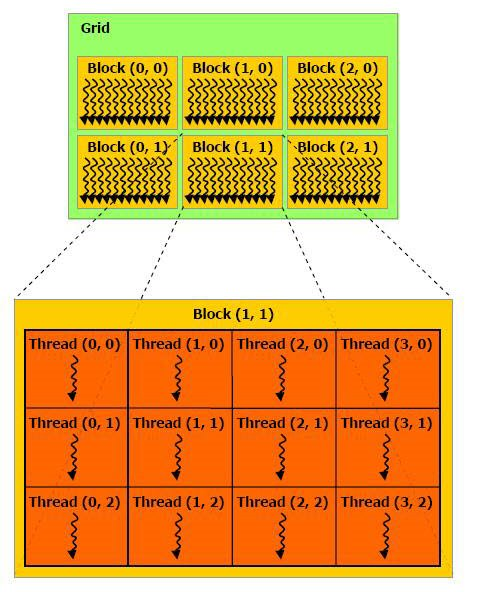
\includegraphics[width=0.8\textwidth]{resources/cudathread.jpg}
        \caption[Organisasi \emph{thread} CUDA]{Organisasi \emph{thread} CUDA \parencite{cuda}}
      \end{figure}

      CUDA \emph{thread} memiliki indeks, yang berdimensi 3. Indeks \emph{thread} akan menunjukkan nomor blok dan nomor \emph{thread} tersebut dalam blok. Menggunakan kedua indeks tersebut, dapat dibentuk nomor yang unik tiap \emph{thread}. Nomor unik tersebut dapat digunakan untuk melakukan pemrosesan paralel pada data besar. Hingga CUDA versi 8.0, maksimum dimensi blok \emph{thread}, dimensi grid, dan jumlah \emph{thread} tiap blok berturut-turut adalah 1024 x 1024 x 64, 65535 x 65535 x 65535, dan 1024.

    \subsubsection{Struktur Memori}

      Tiap \emph{thread} CUDA memiliki memori lokal yang saling independen. Dalam tiap blok, \emph{thread} yang ada dalam blok dapat mengakses \emph{shared memory}. Kemudian ada memori global yang dapat diakses semua \emph{thread}. Ada perbedaan kecepatan ketika melakukan operasi pada tiap tingkatan memori. Urutan kecepatan akses memori yaitu memori lokal, memori bersama, kemudian memori global. Sehingga tidak disarankan menggunakan memori global untuk operasi yang tidak membutuhkan sinkronisasi antar \emph{thread}. Selain itu, ada juga memori yang hanya dapat ditulis oleh \emph{host} yaitu memori konstanta dan tekstur.

\section{Penelitian Terkait}

  \subsection{Rancangan \emph{Multithreading} pada Pencocokan NIDS Berbasis \emph{Signature}} 

    Penelitian terkait optimasi berbasis \emph{multithreading} pada NIDS telah dilakukan oleh \textcite{multi2004}. Tujuan optimasi yaitu untuk meningkatkan kapasitas pencocokan signature. Desain yang diajukan ada 5 buah:

    \begin{enumerate}
      \item \emph{Thread} untuk modul keluaran yang terpisah
      \item Pencocokan signature secara \emph{multithread}
      \item Normalisasi konteks dan pencocokan signature secara \emph{multithread}
      \item Pencegahan \emph{stateful}, normalisasi konteks dan pencocokan signature secara \emph{multithread}
      \item Pencegahan \emph{stateful} secara \emph{multithread} dengan normalisasi konteks dan pencocokan signature secara \emph{multithread} terpisah
    \end{enumerate}

    Hasil yang diperoleh dengan pengukuran pada prosesor Intel Xeon dengan \emph{hyper-threading} menunjukkan bahwa desain 2 dan 3 memiliki kinerja yang rata-rata lebih baik dari pada desain lainnya. Pada desain 2 diperoleh penurunan runtime menjadi 94,1\% dan 86,1\%, untuk menggunakan \emph{hyper-threading enabled} dan tidak. Sedangkan pada desain 3, diperoleh runtime 89\% dan 84\%. Hal ini disebabkan \emph{latency} dari penggunaan \emph{shared memory} pada desain 4 dan 5 yang terlalu besar.

  \subsection{Rancangan NIDS berbasis GPGPU}

    Selain rancangan \emph{multithreading} pada CPU, telah dilakukan penelitian tentang rancangan arsitektur untuk NIDS pada GPGPU \parencite{gnort2008}. Rancangan bertujuan mengakomodasi implementasi algoritma Aho-Corasick pada GPU. Beberapa komponen yang dimodifikasi yaitu implementasi \emph{state machine} dan skema transfer antara \emph{host} dan \emph{device}.

    Implementasi Snort menggunakan struktur memori untuk menyimpan pola \emph{signature} yang berbentuk \emph{list of string}. \emph{Layout} ini kemudian dimodfikasi menjadi \emph{array} 2D sebelum diimplementasi menggunakan CUDA. Kelebihan \emph{layout} memori ini adalah mudah untuk ditransfer ke memori tekstur. Selain itu algoritma Aho-Corasick memanfaatkan prinsip \emph{locality} dengan baik. Sehingga implementasi memori dapat meningkatkan kinerja pencocokan NIPS hingga 19\%.

    Transfer data dari \emph{host} ke \emph{device} maupun \emph{device} ke \emph{host} menggunakan skema \emph{double buffering}. Skema ini menggunakan sebuah \emph{buffer} untuk menampung paket yang ingin dicek menjadi satu batch besar. Batch besar kemudian ditransfer ke memori \emph{device}. Ketika GPU melakukan pemrosesan, maka paket yang baru datang akan ditampung dalam \emph{buffer} berbeda. Sehingga kedua \emph{buffer} dapat selalu bertukar posisi. Hal ini mampu meningkatkan utilitas pengiriman rata-rata paket. Selain itu, memori \emph{host} dapat dikonfigurasi menggunakan \emph{pinned memory} agar menurunkan tingkat \emph{memory page swapping} dan juga meningkatkan \emph{throughput} sistem.

    Ada 2 desain pencocokan paket yang diteliti:
    \begin{enumerate}

      \item Pencocokan paralel paket tunggal \\
      Paket akan dibagi menjadi fragmen-fragmen dan disebar merata pada tiap \emph{thread}. Kelebihan dari skema ini yaitu masing-masing \emph{thread} mendapat bagian yang setara dan waktu yang diperlukan untuk pencocokan relatif sama sehingga tidak perlu saling menunggu. Sedangkan kekurangan dari skema ini adalah pencocokan akan mengalami overlap satu sama lain dan perlu penanganan khusus.

      \item Pencocokan paralel multipaket \\
      Masing-masing paket akan didelegasikan pada satu \emph{thread} pada \emph{stream processor}. Kelebihan dari skema ini adalah pencocokan tidak akan mengalami overlap. Sedangkan kekurangan dari skema ini adalah pencocokan harus menunggu satu sama lain karena ukuran paket yang berbeda-beda.

    \end{enumerate}

    Berdasarkan pengujian yang menggunakan 1000 pola acak, pencocokan dengan GPU mendapat \emph{throughput} hingga 2,3 Gbps untuk paket 1500 \emph{byte}. Peningkatan yang berhasil dicapai sebesar 3,2 kali lipat. Spesifikasi lingkungan pengujian yaitu GPU NVIDIA GeForce 8600GT 1,2 GHz dengan 32 stream processor dalam 4 multiprocessor dan memori 512 MB, dan CPU Intel Pentium 4 3,4 Ghz dengan memori 2 GB.

  \subsection{Rancangan NIDS Berbasis \emph{Signature} yang \emph{Scalable} pada GPU}

    Dalam penelitiannya, dijelaskan oleh \textcite{kargus2012} bahwa pada NIDPS, \emph{bottleneck} utama terdapat pada 3 komponen, \emph{packet acquisition}, \emph{multi-string pattern matching}, dan pencocokan opsi \emph{rule}. Pencocokan opsi \emph{rule} hanya dilakukan saat paket terindikasi mengandung serangan oleh tahap multi-string pattern matching. Sebelum PCRE dicocokkan, PCRE akan dipreproses menjadi DFA terlebih dahulu menggunakan algoritma Thompson. Kemudian pencocokan opsi dapat dilakukan menggunakan metode yang serupa dengan pencocokan \emph{multi-string}.

    Salah satu optimasi yang diajukan untuk tahap pencocokan yaitu penggunaan \emph{pipelining}. \emph{Pipelining} dilakukan dengan memisahkan \emph{thread} yang digunakan untuk operasi \emph{I/O} dengan operasi analisis. Kemudian pada tiap operasi \emph{I/O}, akan dilakukan pengumpulan paket dalam \emph{batch} sebelum dilakukan transfer antar komponen. 

    Pengujian dilakukan dengan konfigurasi CPU ganda Intel X5680 dengan 12 core dan dua GPU NVIDIA GTX580. Hasil yang didapatkan menggunakan desain ini mampu mencapai 1,5 sampai 4 kali lipat kinerja Snort. \emph{Latency} dapat menurun hingga 13 mikrodetik pada \emph{offloading} paket awal untuk batch sebesar 1,5 kB. Pada pengujian dengan \emph{traffic} jaringan, rancangan ini mampu mencapai \emph{throughput} 25,2 Gbps pada \emph{input} sebesar 40 Gbps.

  \subsection{Penyimpanan \emph{Signature} dengan Struktur \emph{Trie} Terkompresi}

    Penyimpanan \emph{signature} untuk NIDS dapat dilakukan dengan struktur \emph{trie} terkompresi \parencite{bellekens2014}. Desain utama \emph{trie} menggunakan representasi penelusuran \emph{breadth first search} (BFS). Lokasi \emph{pointer} simpul anak akan dihitung menggunakan \emph{sparse matrix}. Selain itu dilakukan kompresi terhadap bentuk \emph{trie} sehingga memori yang dibutuhkan lebih padat.

    Masing-masing simpul dalam \emph{trie} akan mengandung tiga buah informasi, matriks akan berisi \emph{offset} dari lokasi simpul anak terkecil dan sebuah \emph{bitmap} berisi flag dari semua simpul anak dalam 256 karakter ASCII. Ketika ingin melakukan penelusuran, simpul akan melakukan penghitungan karakter berdasarkan offset pertama simpul ditambah dengan kumulatif dari tiap bit.

    Optimasi berikutnya yaitu kompresi pada suffiks kalimat. Kompresi dilakukan dalam dua tahap: penggabungan pada huruf terakhir dan tiga huruf terakhir yang sama. Huruf terakhir dapat digabungkan karena simpul tersebut tidak memiliki anak lagi. Dan tiap simpul tersebut pasti akan menuju ke penanda akhir string. Jumlah simpul dapat dihitung ulang dengan persamaan berikut: \\
    \begin{equation}
      Q_{final} = Q - \left(\left|P\right| - 1 \right)
    \end{equation} \\
    dengan $Q$ adalah jumlah simpul dan $P$ adalah jumlah pola.

    Kemudian untuk tahap kedua, akan dihitung suffiks dari pola. Tiap suffiks tiga karakter terakhir yang sama akan digabungkan. Jumlah kombinasi dari susunan dua karakter dapat dihitung dengan \\
    \begin{equation}
      r = S^2
    \end{equation} \\
    dengan $r$ adalah jumlah kombinasi susunan dan $S$ adalah banyak huruf yang ada dalam string pola.

    Maka, jumlah kombinasi dari \emph{trie} dapat diestimasi dengan \\
    \begin{equation}
      \overline{L} = 
        \sum_{i=1}^{r} P\left(g = i \right) \cdot 2i =
          \sum_{i=1}^{min\left({r,n} \right)} \frac{\binom{r}{i} \binom{n - i}{i}}{\binom{n}{r}} \cdot 2i
    \end{equation} \\
    dengan $L$ adalah rata-rata panjang \emph{trie} setelah kompresi, $P$ adalah kemungkinan \emph{trie} memiliki suffiks unik sejumlah $i$.
